%\documentclass{standalone}
%\usepackage{tikz}
%\usepackage{pgfplots}

%\begin{document}
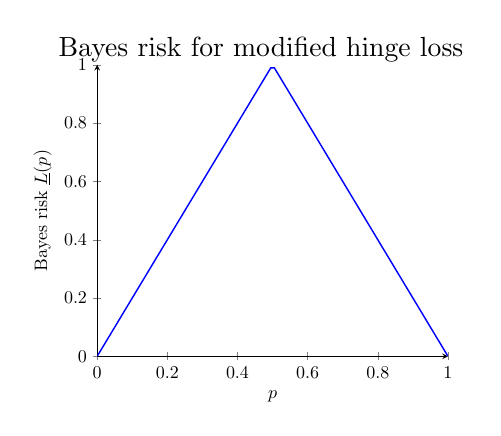
\begin{tikzpicture}[scale=0.65, thick]
    \begin{axis}[
        axis lines = left,
        xlabel = $p$,
        ylabel = Bayes risk $\underline L(p)$,
        xmin = 0,
        xmax = 1,
        ymin = 0,
        ymax =  1,
        grid = none,
    ]
    % Plot the function
    \addplot[
        domain=0.001:0.999,
        samples=100,
        color=blue,
        thick
    ]
    {2 * min(x, 1-x)};
    \end{axis}
    \node at (3.2, 6){Bayes risk for modified hinge loss};
\end{tikzpicture}
%\end{document}
